\problem{Problem 2: Game Show}
    You are a contestant on a new game show, on which you are presented a row
    of $n$ blue chests and a row of~$n$ green chests. The chests in each row are
    numbered from left to right with the numbers $1$ through $n$:
    
    \begin{center}
        \vspace{-1.2em}
        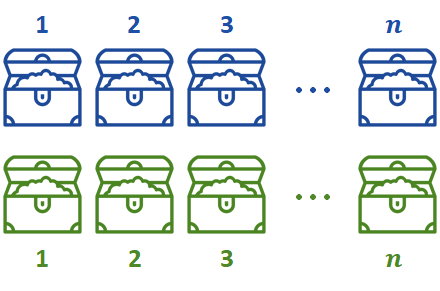
\includegraphics[height=5cm]{chests.png}
        \vspace{-1.2em}
    \end{center}
    
    Each chest has a label
    displaying the amount of prize money (possibly negative!) contained within the chest. For
    $i = 1, \ldots, n$, let $b_i$ denote the prize money in the $i^{\text{th}}$
    blue chest and let $g_i$ denote the prize money in the $i^{\text{th}}$
    green chest. Your goal is to choose the best combination of chests to open
    to maximize your total prize money (i.e., the sum of the prize money in the
    chests you opened). The rules of the game are as follows:
    \begin{itemize}
        \item You must open chests in a left-to-right order and you can open
        {\em at most} one chest in each column. You are
        {\em not} required to open a chest in every column.
        
        \item You must alternate between opening blue chests and green chests.
        In other words, 
        no consecutively-{\em chosen} chests can belong to the same row.
        For example, if you chose chest $b_i$, skipped columns $i+1$ and $i+2$, and chose a chest from column $i+3$, then you must have selected $g_{i+3}$. 
        You may choose {\em any} chest to be the first chest you open.
    \end{itemize}
    Give a dynamic programming algorithm for computing the maximum prize money
    you can earn. The running time of your algorithm must be a polynomial in $n$.
    
    An example problem instance with accompanying solution (27) is illustrated below:
    \[ 
        \begin{array}{c|ccccccc}
            i   & 1 & 2 & 3 & 4 & 5 & 6 & 7 \\ \hline
            b_i & 1 & \fbox{$-1$} & -2 & 3 & 3 & \fbox{10} & -2 \\
            g_i & \fbox{8} & 1 & 4 & \fbox{10} & 2 & 6 & -4
        \end{array}
    \]


\paragraph{Recursive Structure.}
Explain the optimal substructure for this problem. This should make it clear what choices are available for solving a large problem and which subproblems result from each choice.

%TODO: Provide recursive structure of your algorithm
Starting from the end of the array index, there are three choices one could make: choosing the green chest, choosing the blue chest, or skipping the index. For every index before the last index, there are two choices available: choosing the opposite color from the previous index or skipping the index. Choose the greater value from these two options. Taking into account these choices would make every problem's substructures optimal. 


\paragraph{Memory.}
Describe the structure of the memory you'll be using to keep track of solutions to subproblems. Be sure to mention, asymptotically, the size of this memory.

%TODO: Describe memory your algorithm will use
The memory this algorithm uses is a $2*n$ matrix. For each recursive function call, there are two parameters (index and color) that specify the position of chest the function is operating on. There are two colors in total, so a memoization of size 2*n would store all outcomes for subproblems.

\paragraph{Algorithm.}
Describe your dynamic programming algorithm using the recursive structure and the memory you provided above.

%TODO: Describe your algorithm
Initialize the memory as a $2*n$ matrix with value 1.1(default value to differentiate from integers).
The recursive function call takes two parameters: color and index.\newline
First check in the memory if this position has already been assigned a value.If true, return the value at the position in the memory. \newline
Then, check for the base case: if $index == 1$, return the greater value between 0 and the value of the chest this function call is looking at.
If the function is not at its base case, consider the two options: \newline
1. skip this index and continue to $index - 1$, denoted by skip = 0 + Func(color, $index - 1$). \newline
2. choose to open the chest and continue to $index - 1$, denoted by choose  = grid[color][index] + Func(the other color, $index - 1$)\newline
Store the greater value between skip and choose to the memory according to color and index, and then return this value. \newline
Call the function twice: Func(blue, index) and Func(green, index), and return the greater value between these two.


\paragraph{Running Time.}
Analyze, asymptotically, the worst-case running time of your algorithm.

%TODO: Provide and justify the running time of your algorithm
The worst-case running time of this algorithm is O(n). Since the size of the memory is $2*n$, this algorithm would take $2*n$ time to fill up the memory for the non-recursive work of each function call, and accessing each position in the memory after it has been filled would require constant time to read the value. Ignoring the constant $2$ for the worst-case, the running time is O(n).